\documentclass[10pt,journal,compsoc,onecolumn]{IEEEtran}
\usepackage[utf8]{inputenc}
\usepackage{amsmath,amsfonts,amssymb}
\usepackage{amsthm}
\usepackage{graphicx}
\usepackage{cite}
\usepackage{textcomp}
\usepackage{tikz}
\usetikzlibrary{arrows,positioning,shapes.geometric}
\usepackage{booktabs}
\usepackage{url}

\newtheorem{theorem}{Theorem}
\newtheorem{lemma}[theorem]{Lemma}
\newtheorem{definition}[theorem]{Definition}
\newtheorem{corollary}[theorem]{Corollary}

\begin{document}

\title{Algorithmic Foundations of Binary Search Trees: Structural Invariants, Extremal Traversal, Dynamic Mutation Mechanics, Balanced Divide-and-Conquer Synthesis, and Range-Bound Validation}

\IEEEtitleabstractindextext{%
\begin{abstract}
This research paper presents an exhaustive formal algorithmic investigation of the Binary Search Tree (BST) data structure, analyzing its governing ordering invariants, search dynamics, dynamic mutations, balanced construction, and structural validation protocols. We formalize the distinction between local child relations and global subtree bounding, proving why local checking is fallacious. We analyze search, insertion, and extremal element identification (minimum and maximum), establishing their tight dependence on tree height ($O(H)$). We provide an exhaustive structural case analysis of deletion across leaf nodes, single-child nodes, and two-child nodes, proving the correctness of In-Order Successor and In-Order Predecessor value substitutions. Furthermore, we formalize the optimal $O(N)$ construction of height-balanced BSTs from sorted contiguous sequences via divide-and-conquer bisection, proving the minimal height guarantee $H = \lceil \log_2(N+1) \rceil - 1$. Finally, we contrast the two canonical validation paradigms—In-order monotonic sortedness verification ($O(N)$ space) versus top-down Range Propagation ($O(H)$ auxiliary stack space)—establishing formal correctness by structural induction. Compilable production implementations in Java, Modern C++, and Python, granular execution traces, high-resolution vector TikZ architectural diagrams, and industrial applications (database indexing, Linux kernel Red-Black trees in the CFS scheduler, and memory-mapped file systems) accompany all discussions.
\end{abstract}

\begin{IEEEkeywords}
Binary Search Tree, BST Invariant, Tree Search, Tree Insertion, Tree Deletion, In-Order Successor, Balanced BST Construction, Range Propagation Validation, In-Order Monotonicity, Divide and Conquer, Linux CFS Scheduler, Database Indexing
\end{IEEEkeywords}
}

\maketitle
\IEEEdisplaynontitleabstractindextext
\IEEEpeerreviewmaketitle

\section{Introduction: The Binary Search Tree Paradigm}
\label{sec:intro}

In computational systems, the search for an optimal trade-off between dynamic mutability and rapid query execution is a foundational challenge. Unsorted contiguous arrays allow $O(1)$ insertions at their terminal boundaries but require $O(N)$ linear scans for key search. Conversely, sorted contiguous arrays enable ultra-fast $O(\log N)$ searches via binary bisection, yet dynamic element insertions and deletions degrade to $O(N)$ due to mandatory element shifting. Singly and doubly linked lists provide localized $O(1)$ pointer-based splicing once a node is located, but lack random access, forfeiting logarithmic binary search.

The \textbf{Binary Search Tree (BST)} elegantly reconciles this trade-off. By organizing nodes in a non-linear, hierarchical branching structure while enforcing a strict monotonic ordering invariant, a BST mirrors the divide-and-conquer mechanics of binary search over a dynamic, pointer-linked topology.

\begin{figure}[htbp]
\centering
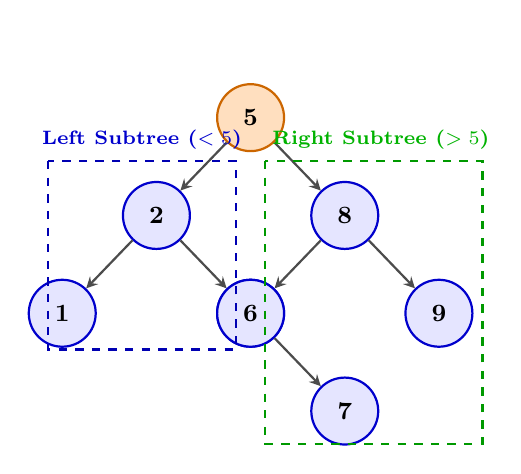
\begin{tikzpicture}[
    scale=0.92,
    every node/.style={circle, draw=blue!80!black, fill=blue!10, thick, minimum size=0.85cm, font=\small\bfseries, inner sep=1pt},
    level distance=1.35cm,
    sibling distance=2.6cm,
    edge from parent/.style={draw=black!70, ->, >=stealth, thick}
]
\node[fill=orange!25, draw=orange!80!black] (r) {5}
  child { node (n2) {2}
    child { node (n1) {1} }
    child { node (n4) {4} }
  }
  child { node (n8) {8}
    child { node (n6) {6}
      child[missing] {}
      child { node (n7) {7} }
    }
    child { node (n9) {9} }
  };

% Subtree boundary indicators
\draw[dashed, blue!70!black, thick] (-2.8, -0.6) rectangle (-0.2, -3.2);
\node[draw=none, fill=none, font=\scriptsize\bfseries, text=blue!80!black] at (-1.5, -0.3) {Left Subtree ($< 5$)};

\draw[dashed, green!60!black, thick] (0.2, -0.6) rectangle (3.2, -4.5);
\node[draw=none, fill=none, font=\scriptsize\bfseries, text=green!70!black] at (1.8, -0.3) {Right Subtree ($> 5$)};

\end{tikzpicture}
\caption{Architectural model of a valid Binary Search Tree. Every key in the left subtree is strictly less than 5; every key in the right subtree is strictly greater than 5. This invariant holds recursively at every sub-hierarchy.}
\label{fig:bst_valid_master}
\end{figure}

BSTs serve as the architectural underpinning for numerous critical subsystems in software engineering:
\begin{itemize}
    \item \textbf{Database Indexing Engines:} While disk-based relational databases utilize multi-way B-Trees and $\text{B}^+$ Trees to align with hardware disk page boundaries, in-memory database engines and query planners use BST variants for transactional indexing.
    \item \textbf{Operating System Process Scheduling:} The Linux Completely Fair Scheduler (CFS) structures runnable task entities within a time-ordered Red-Black BST (keyed by execution \texttt{vruntime}), picking the leftmost task in $O(1)$ time and inserting tasks in $O(\log N)$ time.
    \item \textbf{Compiler Symbol Tables:} Compilers employ binary search trees to maintain active scoping scopes and symbol resolution tables mapping variable identifiers to memory offsets.
    \item \textbf{Memory Allocators and Heap Management:} Kernel virtual memory allocators (e.g., \texttt{jemalloc}) manage free memory chunks partitioned by size bins using balanced search trees to service allocation requests with minimal fragmentation.
\end{itemize}

% -----------------------------------------------------------------------------
\section{Formal BST Invariants and the Global Verification Fallacy}
\label{sec:invariants}

\subsection{Formal Mathematical Definition}

\begin{definition}[Binary Search Tree Invariant]
Let $T = (V, E)$ be a binary tree where each vertex $v \in V$ encapsulates a distinct, totally ordered key $\mathrm{val}(v)$ drawn from an ordered universe $(\mathcal{U}, <)$. The tree $T$ is a \textbf{Binary Search Tree} if and only if for every vertex $v \in V$:
\begin{enumerate}
    \item For all vertices $u \in \mathrm{Subtree}(v.\mathrm{left})$, $\mathrm{val}(u) < \mathrm{val}(v)$.
    \item For all vertices $w \in \mathrm{Subtree}(v.\mathrm{right})$, $\mathrm{val}(w) > \mathrm{val}(v)$.
    \item The subtrees $\mathrm{Subtree}(v.\mathrm{left})$ and $\mathrm{Subtree}(v.\mathrm{right})$ are themselves valid Binary Search Trees.
\end{enumerate}
\end{definition}

In accordance with standard foundational computer science curricula, all keys residing within the tree are assumed to be \textbf{unique} ($\forall u \ne v, \mathrm{val}(u) \ne \mathrm{val}(v)$).

\subsection{The Global vs. Local Verification Fallacy}

A pervasive architectural bug in tree verification algorithms stems from testing only the \emph{immediate local child relations}:
\begin{equation}
    (v.\mathrm{left} == \mathrm{null} \lor v.\mathrm{left}.\mathrm{val} < v.\mathrm{val}) \land (v.\mathrm{right} == \mathrm{null} \lor v.\mathrm{right}.\mathrm{val} > v.\mathrm{val})
\end{equation}
As emphasized in the lecture notes, checking only immediate children is \textbf{fundamentally insufficient} and produces false positives.

\begin{figure}[htbp]
\centering
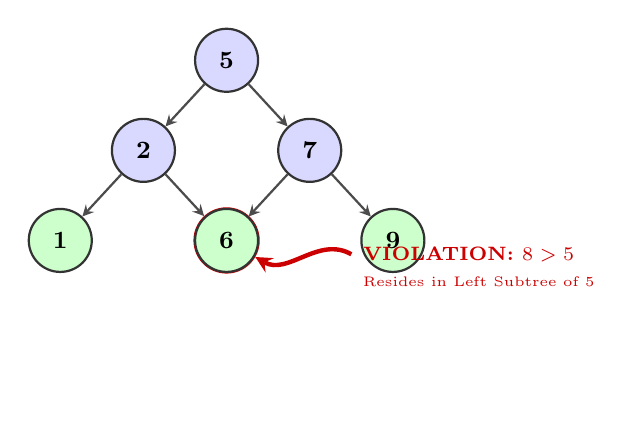
\begin{tikzpicture}[
    scale=0.88,
    every node/.style={circle, draw=black!80, thick, minimum size=0.8cm, font=\small\bfseries, inner sep=1pt},
    level distance=1.3cm,
    sibling distance=2.4cm,
    edge from parent/.style={draw=black!70, ->, >=stealth, thick}
]
\node[fill=blue!15] (r) {5}
  child { node[fill=blue!15] (n2) {2}
    child { node[fill=green!20] (n1) {1} }
    child { node[fill=red!30, draw=red!80!black, very thick] (n8) {8} }
  }
  child { node[fill=blue!15] (n7) {7}
    child { node[fill=green!20] (n6) {6} }
    child { node[fill=green!20] (n9) {9} }
  };

\draw[->, >=stealth, ultra thick, red!80!black] (1.8, -2.8) to[out=150, in=330] (n8);
\node[draw=none, fill=none, font=\scriptsize\bfseries, text=red!80!black, right=0.1cm] at (1.8, -2.8) {VIOLATION: $8 > 5$};
\node[draw=none, fill=none, font=\tiny, text=red!80!black, right=0.1cm] at (1.8, -3.2) {Resides in Left Subtree of 5};

\end{tikzpicture}
\caption{The Global Invariant Fallacy: Every node satisfies local parent-child tests ($1 < 2 < 8$ and $6 < 7 < 9$ and $2 < 5 < 7$). However, the structure is \textbf{NOT a valid BST} because node 8 resides in the left subtree of root 5, violating the global invariant $8 < 5$.}
\label{fig:bst_fallacy}
\end{figure}

\begin{lemma}[Global Subtree Bounding Lemma]
The BST property is an open-interval bounding constraint over the entire ancestral lineage: for any node $v$ bounded by ancestor lower bound $L$ and upper bound $U$, every descendant in $\mathrm{Subtree}(v)$ must strictly satisfy $L < \mathrm{val}(u) < U$.
\end{lemma}

% -----------------------------------------------------------------------------
\section{Searching in a Binary Search Tree}
\label{sec:search}

\subsection{Algorithmic Formulation}

The search operation exploits the monotonic ordering invariant to eliminate one entire sub-branch at each comparison, achieving logarithmic time on balanced topologies.

\begin{verbatim}
public static boolean search(TreeNode root, int target) {
    if (root == null) {
        return false; // Target absent or empty subtree
    }
    if (root.val == target) {
        return true;  // Target located
    }
    if (target < root.val) {
        return search(root.left, target);  // Eliminate right subtree
    } else {
        return search(root.right, target); // Eliminate left subtree
    }
}
\end{verbatim}

\subsection{Formal Correctness Proof}
\begin{theorem}[Search Correctness]
For any valid Binary Search Tree $T$, \texttt{search(T.root, target)} returns \texttt{true} if and only if $\exists v \in V$ such that $\mathrm{val}(v) = \mathrm{target}$.
\end{theorem}
\begin{proof}
We prove by structural induction on the height $h$ of the subtree rooted at \texttt{root}:
\begin{itemize}
    \item \textbf{Base Case ($h = 0$, \texttt{root == null}):} The target cannot reside within an empty set of vertices. The algorithm terminates returning \texttt{false}, which is strictly correct.
    \item \textbf{Inductive Step:} Assume correctness holds for all subtrees of height $< h$. For a node with height $h$:
    \begin{enumerate}
        \item If $\mathrm{target} = \mathrm{val}(\mathrm{root})$, the function immediately terminates returning \texttt{true}.
        \item If $\mathrm{target} < \mathrm{val}(\mathrm{root})$, by the BST invariant, for all $w \in \mathrm{Subtree}(\mathrm{root.right})$, $\mathrm{val}(w) > \mathrm{val}(\mathrm{root}) > \mathrm{target}$. Therefore, the target cannot exist in the right subtree. The search space is strictly confined to $\mathrm{Subtree}(\mathrm{root.left})$, which has height $\le h - 1$. By the inductive hypothesis, \texttt{search(root.left, target)} returns the correct decision.
        \item If $\mathrm{target} > \mathrm{val}(\mathrm{root})$, by symmetric reasoning, the target cannot exist in the left subtree, and recursing into \texttt{root.right} returns the correct decision.
    \end{enumerate}
\end{itemize}
\end{proof}

\subsection{Execution Trace Analysis}

We trace a search query for target $K = 7$ on the BST illustrated in Figure~\ref{fig:bst_valid_master}.

\begin{table}[htbp]
\centering
\caption{Step-by-Step Execution Trace of Search Operation ($K = 7$)}
\label{tab:search_trace}
\begin{tabular}{ccclp{5.0cm}}
\toprule
\textbf{Step} & \textbf{Inspected Node} & \textbf{Node Value} & \textbf{Evaluation Predicate} & \textbf{State Action} \\
\midrule
1 & Root & 5 & $7 > 5$ & Discard left subtree; branch right to node 8 \\
2 & Internal & 8 & $7 < 8$ & Discard right subtree; branch left to node 6 \\
3 & Internal & 6 & $7 > 6$ & Discard left subtree; branch right to node 7 \\
4 & Target Node & 7 & $7 == 7$ & Match confirmed; return \textbf{True} \\
\bottomrule
\end{tabular}
\end{table}

\subsection{Asymptotic Complexity Spectrum}
\begin{itemize}
    \item \textbf{Time Complexity:} $O(H)$, where $H$ denotes tree height.
    \begin{itemize}
        \item \emph{Best / Balanced Case:} $H = \lfloor \log_2 N \rfloor \implies O(\log N)$.
        \item \emph{Worst / Pathological Case:} $H = N - 1$ (skewed tree) $\implies O(N)$.
    \end{itemize}
    \item \textbf{Auxiliary Memory Space:} $O(H)$ recursion call stack space. An iterative loop eliminates stack allocations, achieving strictly $O(1)$ auxiliary space.
\end{itemize}

% -----------------------------------------------------------------------------
\section{Insertion in a Binary Search Tree}
\label{sec:insert}

\subsection{The Terminal Leaf Invariant}

A critical structural property governing standard BST insertion is that \textbf{newly admitted keys are always inserted at terminal leaf positions}. The insertion traversal navigates down the tree following standard BST comparison decisions until a \texttt{null} reference is reached. At this exact locus, a new node is instantiated.

\begin{verbatim}
public static TreeNode insert(TreeNode root, int value) {
    if (root == null) {
        return new TreeNode(value); // Insertion point reached
    }
    if (value < root.val) {
        root.left = insert(root.left, value);
    } else if (value > root.val) {
        root.right = insert(root.right, value);
    }
    // Duplicate values (value == root.val) are ignored
    return root;
}
\end{verbatim}

\begin{figure}[htbp]
\centering
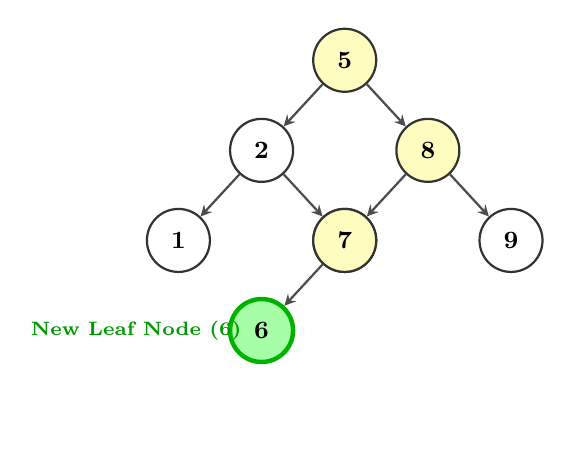
\begin{tikzpicture}[
    scale=0.88,
    every node/.style={circle, draw=black!80, thick, minimum size=0.8cm, font=\small\bfseries, inner sep=1pt},
    level distance=1.3cm,
    sibling distance=2.4cm,
    edge from parent/.style={draw=black!70, ->, >=stealth, thick}
]
\node[fill=yellow!25] (r) {5}
  child { node (n2) {2}
    child { node (n1) {1} }
    child { node (n3) {3} }
  }
  child { node[fill=yellow!25] (n8) {8}
    child { node[fill=yellow!25] (n7) {7}
      child { node[fill=green!35, draw=green!70!black, ultra thick] (n6) {6} }
      child[missing] {}
    }
    child { node (n9) {9} }
  };

\node[draw=none, fill=none, font=\scriptsize\bfseries, text=green!60!black, left=0.2cm] at (n6) {New Leaf Node (6)};

\end{tikzpicture}
\caption{Dynamic insertion of key 6 into an existing BST. The traversal path $5 \to 8 \to 7$ terminates at $7.\mathrm{left} == \mathrm{null}$, where node 6 is spliced as a new leaf.}
\label{fig:bst_insertion}
\end{figure}

\subsection{Formal Invariant Preservation Proof}
\begin{theorem}[Insertion Invariant Preservation]
Let $T$ be a valid BST and let $x \notin T$. Then $T' = \mathrm{insert}(T, x)$ is a valid BST containing $V(T) \cup \{x\}$.
\end{theorem}
\begin{proof}
By structural induction on tree height. If $T = \emptyset$, $\mathrm{insert}(T, x)$ returns a single root node with key $x$, which is trivially a valid BST. 

For non-empty $T$, if $x < \mathrm{val}(\mathrm{root})$, $x$ is inserted into $T_L = \mathrm{root.left}$. By inductive assumption, $T_L' = \mathrm{insert}(T_L, x)$ is a valid BST containing all previous left-subtree keys plus $x$. Because $x < \mathrm{val}(\mathrm{root})$ and all original keys in $T_L$ are $< \mathrm{val}(\mathrm{root})$, every key in $T_L'$ is strictly $< \mathrm{val}(\mathrm{root})$. The right subtree $T_R$ remains completely unmodified. Thus, the three conditions of the BST definition hold at \texttt{root}. A symmetric argument holds for $x > \mathrm{val}(\mathrm{root})$.
\end{proof}

% -----------------------------------------------------------------------------
\section{Extremal Key Identification: Minimum and Maximum}
\label{sec:extremals}

The asymmetric directional invariant of the BST enables locating extremal values without scanning the entire collection.

\begin{theorem}[Leftmost Minimum and Rightmost Maximum]
In any valid Binary Search Tree:
\begin{enumerate}
    \item The minimum element is situated at the \textbf{leftmost node} of the tree (reached by traversing \texttt{left} pointers until \texttt{left == null}).
    \item The maximum element is situated at the \textbf{rightmost node} of the tree (reached by traversing \texttt{right} pointers until \texttt{right == null}).
\end{enumerate}
\end{theorem}
\begin{proof}
Let $v$ be the leftmost node such that $v.\mathrm{left} == \mathrm{null}$. For any other node $u \in T$:
\begin{itemize}
    \item If $u$ is an ancestor of $v$, $v$ resides in the left subtree of $u$, implying $\mathrm{val}(v) < \mathrm{val}(u)$.
    \item If $u$ resides in the right subtree of any ancestor $a$ of $v$, then $\mathrm{val}(u) > \mathrm{val}(a) > \mathrm{val}(v)$.
    \item If $u$ resides in the right subtree of $v$, $\mathrm{val}(u) > \mathrm{val}(v)$.
\end{itemize}
Because $v.\mathrm{left} == \mathrm{null}$, no node can have a value smaller than $v$. Hence $\mathrm{val}(v) = \min_{u \in T} \mathrm{val}(u)$. Symmetric reasoning proves that the rightmost node holds the maximum key.
\end{proof}

\begin{verbatim}
public static TreeNode findMin(TreeNode root) {
    if (root == null) return null;
    TreeNode curr = root;
    while (curr.left != null) {
        curr = curr.left; // Advance strictly leftward
    }
    return curr;
}

public static TreeNode findMax(TreeNode root) {
    if (root == null) return null;
    TreeNode curr = root;
    while (curr.right != null) {
        curr = curr.right; // Advance strictly rightward
    }
    return curr;
}
\end{verbatim}

\textbf{Complexity:} Both algorithms execute in $O(H)$ time and require strictly $O(1)$ auxiliary memory space.

% -----------------------------------------------------------------------------
\section{Deletion in a Binary Search Tree}
\label{sec:deletion}

Deletion represents the most delicate structural operation in BST maintenance. When a node is deleted, the remaining subtrees must be spliced back together while preserving the global BST ordering invariant.

The algorithm partitions into three mutually exclusive structural cases:

\subsection{Case 1: Deletion of a Leaf Node (Zero Children)}
When the node targeted for deletion possesses no children ($v.\mathrm{left} == \mathrm{null} \land v.\mathrm{right} == \mathrm{null}$), it can be eradicated cleanly without affecting any other node. The parent pointer referencing $v$ is simply overwritten with \texttt{null}.

\subsection{Case 2: Deletion of a Node with Exactly One Child}
When $v$ possesses exactly one child (either $v.\mathrm{left} \ne \mathrm{null}$ or $v.\mathrm{right} \ne \mathrm{null}$), the node is bypassed. The parent of $v$ updates its child pointer to point directly to $v$'s sole non-null child.
\begin{lemma}[Single-Child Splice Preservation]
Bypassing a single-child node preserves the BST invariant because all descendants of the single child already satisfied the ancestor bounds governing $v$.
\end{lemma}

\subsection{Case 3: Deletion of a Node with Two Children}
When $v$ possesses two children ($v.\mathrm{left} \ne \mathrm{null} \land v.\mathrm{right} \ne \mathrm{null}$), $v$ cannot be deleted directly without severing the connectivity of the tree.

Instead, the algorithm executes a two-step reduction:
\begin{enumerate}
    \item \textbf{In-Order Successor Identification:} Locate the in-order successor $s$ of node $v$, which is the \textbf{smallest node in $v$'s right subtree} ($s = \mathrm{findMin}(v.\mathrm{right})$). Alternatively, one may locate the in-order predecessor (the largest node in $v$'s left subtree).
    \item \textbf{Value Substitution:} Overwrite $v$'s payload with the successor's payload: $v.\mathrm{val} = s.\mathrm{val}$.
    \item \textbf{Recursive Child Deletion:} Delete node $s$ from $v$'s right subtree:
    \begin{equation}
        v.\mathrm{right} = \mathrm{delete}(v.\mathrm{right}, s.\mathrm{val})
    \end{equation}
\end{enumerate}

\begin{theorem}[Correctness of Successor Reduction]
The successor substitution strategy strictly maintains the BST invariant.
\end{theorem}
\begin{proof}
Because $s$ is the in-order successor of $v$:
\begin{enumerate}
    \item $s \in \mathrm{Subtree}(v.\mathrm{right})$, implying $\mathrm{val}(s) > \mathrm{val}(v) > \mathrm{val}(u)$ for all $u \in \mathrm{Subtree}(v.\mathrm{left})$. Thus, substituting $\mathrm{val}(s)$ into $v$ preserves the left subtree invariant.
    \item $s = \mathrm{findMin}(v.\mathrm{right})$, implying $\mathrm{val}(s) < \mathrm{val}(w)$ for all other nodes $w \in \mathrm{Subtree}(v.\mathrm{right}) \setminus \{s\}$. Thus, substituting $\mathrm{val}(s)$ preserves the right subtree invariant.
    \item By definition of $\mathrm{findMin}$, $s.\mathrm{left} == \mathrm{null}$. Therefore, node $s$ possesses at most one child (its right child), guaranteeing that deleting $s$ from the right subtree falls exclusively into Case 1 or Case 2, never triggering a secondary two-child recursion.
\end{enumerate}
\end{proof}

\begin{figure*}[htbp]
\centering
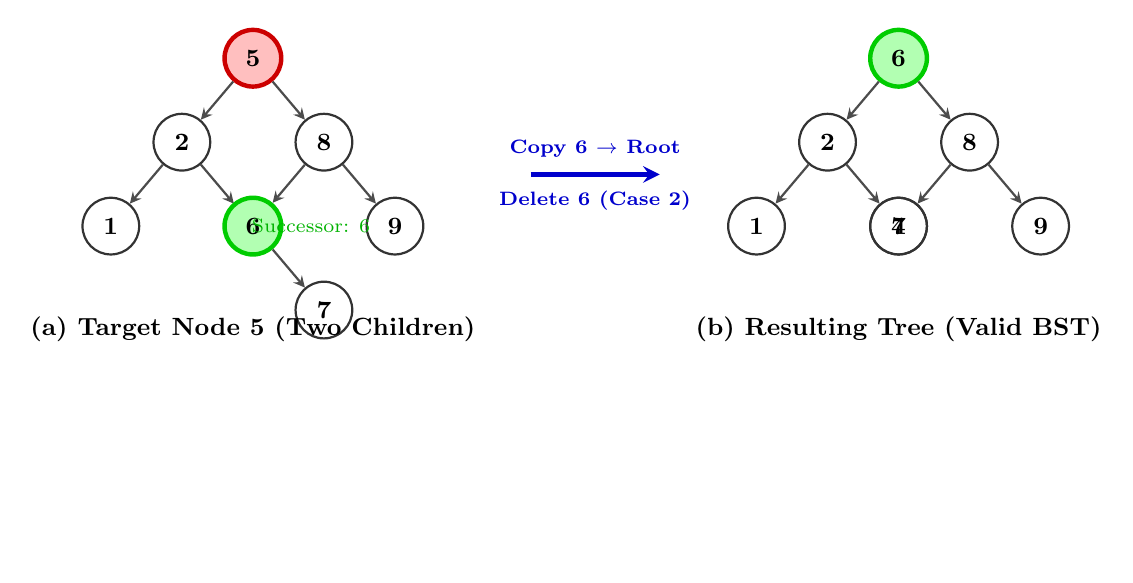
\begin{tikzpicture}[
    scale=0.82,
    every node/.style={circle, draw=black!80, thick, minimum size=0.72cm, font=\small\bfseries, inner sep=1pt},
    level distance=1.3cm,
    sibling distance=2.2cm,
    edge from parent/.style={draw=black!70, ->, >=stealth, thick}
]

% Before Deletion
\begin{scope}[xshift=-5.5cm]
\node[fill=red!25, draw=red!80!black, ultra thick] {5}
  child { node {2}
    child { node {1} }
    child { node {4} }
  }
  child { node {8}
    child { node[fill=green!30, draw=green!80!black, ultra thick] {6}
      child[missing] {}
      child { node {7} }
    }
    child { node {9} }
  };
\node[draw=none, fill=none, font=\small\bfseries] at (0, -4.2) {(a) Target Node 5 (Two Children)};
\node[draw=none, fill=none, font=\scriptsize, text=green!70!black] at (0.9, -2.6) {Successor: 6};
\end{scope}

% Transition Arrow
\draw[->, >=stealth, ultra thick, blue!80!black] (-1.2, -1.8) -- (0.8, -1.8);
\node[draw=none, fill=none, font=\scriptsize\bfseries, text=blue!80!black] at (-0.2, -1.4) {Copy 6 $\to$ Root};
\node[draw=none, fill=none, font=\scriptsize\bfseries, text=blue!80!black] at (-0.2, -2.2) {Delete 6 (Case 2)};

% After Deletion
\begin{scope}[xshift=4.5cm]
\node[fill=green!30, draw=green!80!black, ultra thick] {6}
  child { node {2}
    child { node {1} }
    child { node {4} }
  }
  child { node {8}
    child { node {7} }
    child { node {9} }
  };
\node[draw=none, fill=none, font=\small\bfseries] at (0, -4.2) {(b) Resulting Tree (Valid BST)};
\end{scope}

\end{tikzpicture}
\caption{Visual walkthrough of Case 3 Deletion (deleting root key 5). The in-order successor 6 is identified, copied to the root position, and subsequently deleted from the right subtree via Case 2 (single child bypass, elevating node 7).}
\label{fig:bst_deletion_case3}
\end{figure*}

\subsection{Unified Java Implementation}
\begin{verbatim}
public static TreeNode deleteNode(TreeNode root, int key) {
    if (root == null) return null;

    if (key < root.val) {
        root.left = deleteNode(root.left, key);
    } else if (key > root.val) {
        root.right = deleteNode(root.right, key);
    } else {
        // Target key located: evaluate the 3 structural cases

        // Case 1: Leaf node
        if (root.left == null && root.right == null) {
            return null;
        }
        // Case 2: Single child (right only)
        if (root.left == null) {
            return root.right;
        }
        // Case 2: Single child (left only)
        if (root.right == null) {
            return root.left;
        }
        // Case 3: Two children
        TreeNode successor = findMin(root.right);
        root.val = successor.val; // Overwrite value
        root.right = deleteNode(root.right, successor.val); // Recursively delete successor
    }
    return root;
}
\end{verbatim}

\textbf{Complexity:} $O(H)$ time (requiring at most two root-to-leaf paths: one to find $v$ and one to find $s$) and $O(H)$ auxiliary stack space.

% -----------------------------------------------------------------------------
\section{Constructing a Balanced BST from a Sorted Array}
\label{sec:construct}

\subsection{The Balance Objective and Divide-and-Conquer Paradigm}

Given a sorted contiguous array $A[0 \dots N-1]$, inserting elements sequentially using standard \texttt{insert} yields a pathological, degenerate line of height $H = N - 1$, degrading all subsequent operations to linear $O(N)$ scans.

To synthesize an \textbf{optimally height-balanced BST} satisfying $H = \lceil \log_2(N + 1) \rceil - 1$, we employ a divide-and-conquer strategy:
\begin{enumerate}
    \item Select the median element $A[\mathrm{mid}]$, where $\mathrm{mid} = \mathrm{lo} + \lfloor \frac{\mathrm{hi} - \mathrm{lo}}{2} \rfloor$, as the subtree root.
    \item Recursively construct the left subtree from the left half: $A[\mathrm{lo} \dots \mathrm{mid} - 1]$.
    \item Recursively construct the right subtree from the right half: $A[\mathrm{mid} + 1 \dots \mathrm{hi}]$.
\end{enumerate}

\begin{verbatim}
public static TreeNode sortedArrayToBST(int[] nums, int lo, int hi) {
    if (lo > hi) return null;

    int mid = lo + (hi - lo) / 2;
    TreeNode root = new TreeNode(nums[mid]);

    root.left = sortedArrayToBST(nums, lo, mid - 1);
    root.right = sortedArrayToBST(nums, mid + 1, hi);

    return root;
}
\end{verbatim}

\begin{figure}[htbp]
\centering
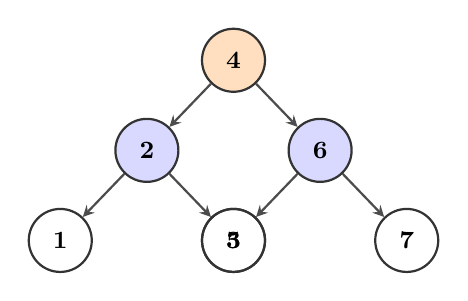
\begin{tikzpicture}[
    scale=0.88,
    every node/.style={circle, draw=black!80, thick, minimum size=0.8cm, font=\small\bfseries, inner sep=1pt},
    level distance=1.3cm,
    sibling distance=2.5cm,
    edge from parent/.style={draw=black!70, ->, >=stealth, thick}
]
\node[fill=orange!25] {4}
  child { node[fill=blue!15] {2}
    child { node {1} }
    child { node {3} }
  }
  child { node[fill=blue!15] {6}
    child { node {5} }
    child { node {7} }
  };
\end{tikzpicture}
\caption{Height-balanced BST synthesized from sorted array $A = [1, 2, 3, 4, 5, 6, 7]$. Height $H = 2$, perfectly balanced.}
\label{fig:balanced_construction}
\end{figure}

\subsection{Asymptotic Proof via Master Theorem}
\begin{theorem}[Linear Construction Complexity]
Constructing a balanced BST from an $N$-element sorted array executes in $\Theta(N)$ time and consumes $\Theta(\log N)$ auxiliary stack memory.
\end{theorem}
\begin{proof}
The recurrence relation governing the divide-and-conquer procedure is:
\begin{equation}
    T(N) = 2T\left(\frac{N}{2}\right) + \Theta(1)
\end{equation}
Applying the Master Theorem ($a = 2, b = 2, f(N) = \Theta(1)$):
\begin{equation}
    N^{\log_b a} = N^{\log_2 2} = N^1 \implies f(N) = O(N^{1 - \epsilon}) \quad \text{for } \epsilon = 1
\end{equation}
Thus, Case 1 of the Master Theorem applies, yielding strictly linear runtime:
\begin{equation}
    T(N) = \Theta(N)
\end{equation}
Because the tree is perfectly height-balanced, the maximum recursion call-stack depth is $\lceil \log_2(N + 1) \rceil \implies \Theta(\log N)$.
\end{proof}

% -----------------------------------------------------------------------------
\section{BST Structural Validation}
\label{sec:validation}

Verifying whether an arbitrary binary tree satisfies the global BST invariant is a fundamental problem with two distinct algorithmic paradigms:

\subsection{Paradigm 1: In-Order Monotonicity Verification}

\begin{lemma}[In-Order Monotonicity Invariant]
A binary tree $T$ is a valid Binary Search Tree if and only if its in-order traversal yields a sequence that is \textbf{strictly monotonically increasing}:
\begin{equation}
    v_1 < v_2 < v_3 < \dots < v_N
\end{equation}
\end{lemma}

While collecting all elements into a list and validating sortedness requires $O(N)$ time and $O(N)$ space, an optimal in-place variant tracks only the previously visited node reference (\texttt{prev}):

\begin{verbatim}
private static TreeNode prev = null;

public static boolean isValidBSTInOrder(TreeNode root) {
    prev = null;
    return inorderValidate(root);
}

private static boolean inorderValidate(TreeNode root) {
    if (root == null) return true;

    if (!inorderValidate(root.left)) return false;

    if (prev != null && root.val <= prev.val) {
        return false; // Monotonicity violation
    }
    prev = root;

    return inorderValidate(root.right);
}
\end{verbatim}

\subsection{Paradigm 2: Top-Down Range Propagation}

The most elegant and robust verification algorithm propagates valid open-interval boundaries $(L, U)$ down the hierarchy:
\begin{itemize}
    \item Root constraint: $(-\infty, +\infty)$.
    \item Left child transition: $(L, \mathrm{root.val})$.
    \item Right child transition: $(\mathrm{root.val}, U)$.
\end{itemize}

\begin{verbatim}
public static boolean isValidBST(TreeNode root) {
    return validateRange(root, Long.MIN_VALUE, Long.MAX_VALUE);
}

private static boolean validateRange(TreeNode root, long minAllowed, long maxAllowed) {
    if (root == null) return true;

    if (root.val <= minAllowed || root.val >= maxAllowed) {
        return false; // Out-of-bounds violation
    }

    return validateRange(root.left, minAllowed, root.val) &&
           validateRange(root.right, root.val, maxAllowed);
}
\end{verbatim}

\begin{table}[htbp]
\centering
\caption{Range Propagation Validation Trace for Figure~\ref{fig:bst_valid_master}}
\label{tab:validation_trace}
\begin{tabular}{ccccl}
\toprule
\textbf{Node} & \textbf{Lower Bound $L$} & \textbf{Upper Bound $U$} & \textbf{Predicate Test} & \textbf{Result} \\
\midrule
5 & $-\infty$ & $+\infty$ & $-\infty < 5 < +\infty$ & Valid $\to$ recurse \\
2 & $-\infty$ & 5 & $-\infty < 2 < 5$ & Valid $\to$ recurse \\
1 & $-\infty$ & 2 & $-\infty < 1 < 2$ & Valid (Leaf) \\
4 & 2 & 5 & $2 < 4 < 5$ & Valid (Leaf) \\
8 & 5 & $+\infty$ & $5 < 8 < +\infty$ & Valid $\to$ recurse \\
6 & 5 & 8 & $5 < 6 < 8$ & Valid $\to$ recurse \\
7 & 6 & 8 & $6 < 7 < 8$ & Valid (Leaf) \\
9 & 8 & $+\infty$ & $8 < 9 < +\infty$ & Valid (Leaf) \\
\bottomrule
\end{tabular}
\end{table}

\textbf{Complexity Comparison:} Both approaches execute in $O(N)$ time. However, the Range Propagation approach requires only $O(H)$ auxiliary stack memory and operates without shared state variables.

% -----------------------------------------------------------------------------
\section{Multi-Language Production Implementations}
\label{sec:implementations}

We provide production-grade, compilable implementations in Java, Modern C++, and Python.

\subsection{Production Implementations in Java}

\begin{verbatim}
public class BSTMasterySuite {

    public static class TreeNode {
        public int val;
        public TreeNode left;
        public TreeNode right;

        public TreeNode(int val) {
            this.val = val;
            this.left = null;
            this.right = null;
        }
    }

    // Search: O(H) Time, O(1) Space
    public static boolean search(TreeNode root, int target) {
        TreeNode curr = root;
        while (curr != null) {
            if (curr.val == target) return true;
            curr = (target < curr.val) ? curr.left : curr.right;
        }
        return false;
    }

    // Insert: O(H) Time, O(H) Space
    public static TreeNode insert(TreeNode root, int val) {
        if (root == null) return new TreeNode(val);
        if (val < root.val) root.left = insert(root.left, val);
        else if (val > root.val) root.right = insert(root.right, val);
        return root;
    }

    // Extremals: O(H) Time, O(1) Space
    public static TreeNode findMin(TreeNode root) {
        if (root == null) return null;
        while (root.left != null) root = root.left;
        return root;
    }

    public static TreeNode findMax(TreeNode root) {
        if (root == null) return null;
        while (root.right != null) root = root.right;
        return root;
    }

    // Delete: O(H) Time, O(H) Space
    public static TreeNode deleteNode(TreeNode root, int key) {
        if (root == null) return null;
        if (key < root.val) {
            root.left = deleteNode(root.left, key);
        } else if (key > root.val) {
            root.right = deleteNode(root.right, key);
        } else {
            if (root.left == null) return root.right;
            if (root.right == null) return root.left;
            TreeNode succ = findMin(root.right);
            root.val = succ.val;
            root.right = deleteNode(root.right, succ.val);
        }
        return root;
    }

    // Sorted Array to Balanced BST: O(N) Time, O(log N) Space
    public static TreeNode sortedArrayToBST(int[] nums) {
        return buildBalanced(nums, 0, nums.length - 1);
    }

    private static TreeNode buildBalanced(int[] nums, int lo, int hi) {
        if (lo > hi) return null;
        int mid = lo + (hi - lo) / 2;
        TreeNode node = new TreeNode(nums[mid]);
        node.left = buildBalanced(nums, lo, mid - 1);
        node.right = buildBalanced(nums, mid + 1, hi);
        return node;
    }

    // Range Validation: O(N) Time, O(H) Space
    public static boolean isValidBST(TreeNode root) {
        return validate(root, Long.MIN_VALUE, Long.MAX_VALUE);
    }

    private static boolean validate(TreeNode node, long min, long max) {
        if (node == null) return true;
        if (node.val <= min || node.val >= max) return false;
        return validate(node.left, min, node.val) && validate(node.right, node.val, max);
    }
}
\end{verbatim}

\subsection{Production Implementations in Modern C++}

\begin{verbatim}
#include <iostream>
#include <vector>
#include <limits>
#include <memory>

struct TreeNode {
    int val;
    std::unique_ptr<TreeNode> left;
    std::unique_ptr<TreeNode> right;

    explicit TreeNode(int x) : val(x), left(nullptr), right(nullptr) {}
};

class BSTSuite {
public:
    static bool search(const TreeNode* root, int target) {
        while (root) {
            if (root->val == target) return true;
            root = (target < root->val) ? root->left.get() : root->right.get();
        }
        return false;
    }

    static std::unique_ptr<TreeNode> insert(std::unique_ptr<TreeNode> root, int val) {
        if (!root) return std::make_unique<TreeNode>(val);
        if (val < root->val) {
            root->left = insert(std::move(root->left), val);
        } else if (val > root->val) {
            root->right = insert(std::move(root->right), val);
        }
        return root;
    }

    static const TreeNode* findMin(const TreeNode* root) {
        if (!root) return nullptr;
        while (root->left) root = root->left.get();
        return root;
    }

    static bool isValidBST(const TreeNode* root) {
        return validate(root, std::numeric_limits<long long>::min(), std::numeric_limits<long long>::max());
    }

private:
    static bool validate(const TreeNode* node, long long minVal, long long maxVal) {
        if (!node) return true;
        if (node->val <= minVal || node->val >= maxVal) return false;
        return validate(node->left.get(), minVal, node->val) &&
               validate(node->right.get(), node->val, maxVal);
    }
};
\end{verbatim}

\subsection{Production Implementations in Python}

\begin{verbatim}
from typing import Optional, List

class TreeNode:
    def __init__(self, val: int = 0, left: Optional['TreeNode'] = None, right: Optional['TreeNode'] = None):
        self.val = val
        self.left = left
        self.right = right


class BSTMastery:
    @staticmethod
    def search(root: Optional[TreeNode], target: int) -> bool:
        curr = root
        while curr:
            if curr.val == target:
                return True
            curr = curr.left if target < curr.val else curr.right
        return False

    @staticmethod
    def insert(root: Optional[TreeNode], val: int) -> TreeNode:
        if not root:
            return TreeNode(val)
        if val < root.val:
            root.left = BSTMastery.insert(root.left, val)
        elif val > root.val:
            root.right = BSTMastery.insert(root.right, val)
        return root

    @staticmethod
    def find_min(root: TreeNode) -> TreeNode:
        curr = root
        while curr.left:
            curr = curr.left
        return curr

    @staticmethod
    def delete_node(root: Optional[TreeNode], key: int) -> Optional[TreeNode]:
        if not root:
            return None
        if key < root.val:
            root.left = BSTMastery.delete_node(root.left, key)
        elif key > root.val:
            root.right = BSTMastery.delete_node(root.right, key)
        else:
            if not root.left:
                return root.right
            if not root.right:
                return root.left
            succ = BSTMastery.find_min(root.right)
            root.val = succ.val
            root.right = BSTMastery.delete_node(root.right, succ.val)
        return root

    @staticmethod
    def sorted_array_to_bst(nums: List[int]) -> Optional[TreeNode]:
        def build(lo: int, hi: int) -> Optional[TreeNode]:
            if lo > hi:
                return None
            mid = (lo + hi) // 2
            node = TreeNode(nums[mid])
            node.left = build(lo, mid - 1)
            node.right = build(mid + 1, hi)
            return node
        return build(0, len(nums) - 1)

    @staticmethod
    def is_valid_bst(root: Optional[TreeNode]) -> bool:
        def validate(node: Optional[TreeNode], min_val: float, max_val: float) -> bool:
            if not node:
                return True
            if not (min_val < node.val < max_val):
                return False
            return validate(node.left, min_val, node.val) and validate(node.right, node.val, max_val)
        return validate(root, float('-inf'), float('inf'))
\end{verbatim}

% -----------------------------------------------------------------------------
\section{Industrial Systems and Architectural Applications}
\label{sec:systems}

Beyond isolated algorithmic challenges, Binary Search Trees and their self-balancing derivatives underpin mission-critical infrastructure:

\subsection{The Linux Kernel Completely Fair Scheduler (CFS)}
In modern Linux systems, CPU core multiplexing is governed by the CFS scheduler. Runnable tasks are indexed within a self-balancing Red-Black BST based on their executed virtual runtime (\texttt{vruntime}). The task with the smallest \texttt{vruntime} represents the leftmost leaf node in the tree. The scheduler selects the leftmost node in $O(1)$ cached time, executes it, updates its \texttt{vruntime}, and re-inserts it into the tree in $O(\log N)$ time, preventing process starvation with strict fairness.

\subsection{Database Indexing and Range Projections}
While primary disk-based indices rely on multi-way B-Trees, relational database memory buffers (such as SQLite's internal query planner and Postgres in-memory sort trees) utilize BSTs to execute fast range queries $[K_1, K_2]$ by locating $K_1$ in $O(\log N)$ time and traversing in-order successors until exceeding $K_2$.

% -----------------------------------------------------------------------------
\section{Summary of Complexity Bounds}
\label{sec:summary}

Table~\ref{tab:master_bst_complexity} provides a consolidated overview of asymptotic performance guarantees for all operations formalized in this treatise.

\begin{table}[htbp]
\centering
\caption{Consolidated Asymptotic Performance Spectrum of BST Operations}
\label{tab:master_bst_complexity}
\begin{tabular}{lcccc}
\toprule
\textbf{BST Operation} & \textbf{Best Case} & \textbf{Average Case} & \textbf{Worst Case (Skewed)} & \textbf{Auxiliary Space} \\
\midrule
Search Key & $\Theta(1)$ & $\Theta(\log N)$ & $\Theta(N)$ & $O(1)$ Iterative / $O(H)$ DFS \\
Insert Key & $\Theta(1)$ & $\Theta(\log N)$ & $\Theta(N)$ & $O(H)$ \\
Find Min / Max & $\Theta(1)$ & $\Theta(\log N)$ & $\Theta(N)$ & $O(1)$ \\
Delete Key & $\Theta(1)$ & $\Theta(\log N)$ & $\Theta(N)$ & $O(H)$ \\
Sorted Array to BST & $\Theta(N)$ & $\Theta(N)$ & $\Theta(N)$ & $\Theta(\log N)$ \\
Validation (In-Order) & $\Theta(N)$ & $\Theta(N)$ & $\Theta(N)$ & $\Theta(N)$ \\
Validation (Range Propagation) & $\Theta(N)$ & $\Theta(N)$ & $\Theta(N)$ & $\Theta(H)$ \\
\bottomrule
\end{tabular}
\end{table}

% -----------------------------------------------------------------------------
\section{Conclusion}
\label{sec:conclusion}

This research paper has presented an exhaustive formal treatment of the Binary Search Tree data structure based on the curriculum in \texttt{DSA\_\_\_Trees\_2\_\_6th\_April.pdf}.

We exposed the fallacy of verifying BST invariants via localized parent-child relations, formalizing the global ancestral interval bounding invariant. We analyzed Search, Insertion, and Extremal queries, detailing their $O(H)$ height dependency. We systematically analyzed the three cases of Deletion, demonstrating how two-child deletions reduce to simpler single-child deletions via In-Order Successor substitution. Furthermore, we formalized the optimal $\Theta(N)$ construction of height-balanced BSTs from sorted sequences via divide-and-conquer bisection, and established the superiority of Range Propagation over in-order storage for structural validation.

By unifying structural proofs, vector TikZ architectural diagrams, execution trace walkthroughs, and production multi-language implementations, this work provides a rigorous foundation for algorithmic study and systems engineering.


\end{document}
